\documentclass[12pt,border=0pt]{standalone}

\usepackage[utf8]{inputenc} 
\usepackage{amssymb,amsmath}
\usepackage{tikz}
\usepackage{nicefrac}



\thispagestyle{empty}

\begin{document}

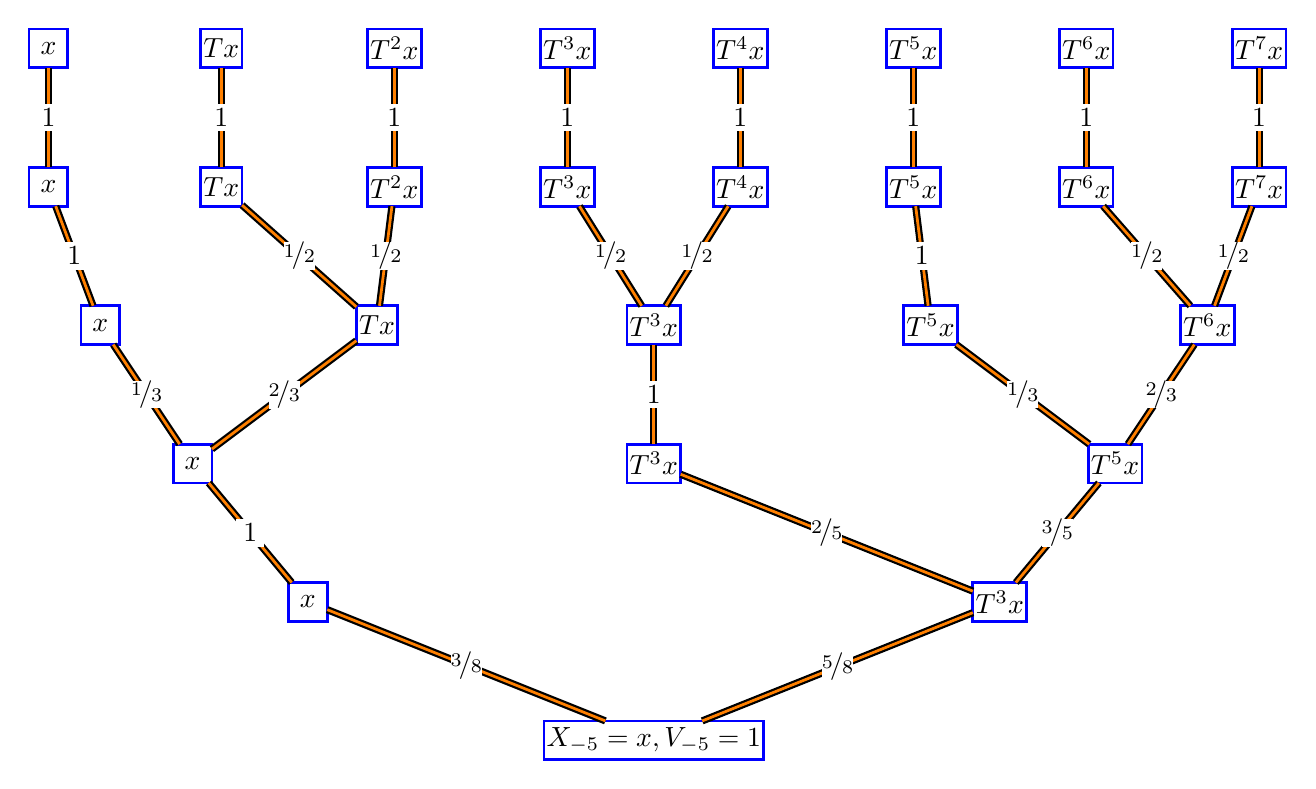
\begin{tikzpicture}[x=10pt,y=6pt]
  \centering
  \tikzset{VertexStyle/.style = {
    shape         = rectangle,
    draw          = blue, 
    fill          = white, 
  	line width    = 1pt, 
    text          = black,
    inner sep     = 1pt,
    outer sep     = 0pt,
    minimum size  = 14 pt,
    scale         = 1
    }
  }
  \tikzset{EdgeStyle/.style = {
    draw            = black, 
    thick,
    double          = orange,
    double distance = 1pt
    }
  }
  \tikzset{EdgeLabelStyle/.style = {
    draw          = none,
  	shape         = rectangle, 
  	line width    = 1pt, 
  	minimum size  = 10pt, 
    inner sep     = 0pt,
    outer sep     = 0pt,
    fill          = white,
    text          = black,
    scale         = 1
    }
  }

	\node[VertexStyle](A1) at (25, 0) {$X_{-5} = x, V_{-5}=1$};
	\node[VertexStyle](B1) at (12.5, 8.33333333333333) {$x$};
	\node[VertexStyle](B2) at (37.5, 8.33333333333333) {$T^3x$};
	\node[VertexStyle](C1) at (8.33333333333333, 16.6666666666667) {$x$};
	\node[VertexStyle](C2) at (25, 16.6666666666667) {$T^3x$};
	\node[VertexStyle](C3) at (41.6666666666667, 16.6666666666667) {$T^5x$};
	\node[VertexStyle](D1) at (5, 25) {$x$};
	\node[VertexStyle](D2) at (15, 25) {$Tx$};
	\node[VertexStyle](D3) at (25, 25) {$T^3x$};
	\node[VertexStyle](D4) at (35, 25) {$T^5x$};
	\node[VertexStyle](D5) at (45, 25) {$T^6x$};
	\node[VertexStyle](E1) at (3.125, 33.3333333333333) {$x$};
	\node[VertexStyle](E2) at (9.375, 33.3333333333333) {$Tx$};
	\node[VertexStyle](E3) at (15.625, 33.3333333333333) {$T^2x$};
	\node[VertexStyle](E4) at (21.875, 33.3333333333333) {$T^3x$};
	\node[VertexStyle](E5) at (28.125, 33.3333333333333) {$T^4x$};
	\node[VertexStyle](E6) at (34.375, 33.3333333333333) {$T^5x$};
	\node[VertexStyle](E7) at (40.625, 33.3333333333333) {$T^6x$};
	\node[VertexStyle](E8) at (46.875, 33.3333333333333) {$T^7x$};
	\node[VertexStyle](F1) at (3.125, 41.6666666666667) {$x$};
	\node[VertexStyle](F2) at (9.375, 41.6666666666667) {$Tx$};
	\node[VertexStyle](F3) at (15.625, 41.6666666666667) {$T^2x$};
	\node[VertexStyle](F4) at (21.875, 41.6666666666667) {$T^3x$};
	\node[VertexStyle](F5) at (28.125, 41.6666666666667) {$T^4x$};
	\node[VertexStyle](F6) at (34.375, 41.6666666666667) {$T^5x$};
	\node[VertexStyle](F7) at (40.625, 41.6666666666667) {$T^6x$};
	\node[VertexStyle](F8) at (46.875, 41.6666666666667) {$T^7x$};
	\draw[EdgeStyle](A1) to node[EdgeLabelStyle]{$\nicefrac{3}{8}$} (B1);
	\draw[EdgeStyle](A1) to node[EdgeLabelStyle]{$\nicefrac{5}{8}$} (B2);
	\draw[EdgeStyle](B1) to node[EdgeLabelStyle]{$1$} (C1);
	\draw[EdgeStyle](B2) to node[EdgeLabelStyle]{$\nicefrac{2}{5}$} (C2);
	\draw[EdgeStyle](B2) to node[EdgeLabelStyle]{$\nicefrac{3}{5}$} (C3);
	\draw[EdgeStyle](C1) to node[EdgeLabelStyle]{$\nicefrac{1}{3}$} (D1);
	\draw[EdgeStyle](C1) to node[EdgeLabelStyle]{$\nicefrac{2}{3}$} (D2);
	\draw[EdgeStyle](C2) to node[EdgeLabelStyle]{$1$} (D3);
	\draw[EdgeStyle](C3) to node[EdgeLabelStyle]{$\nicefrac{1}{3}$} (D4);
	\draw[EdgeStyle](C3) to node[EdgeLabelStyle]{$\nicefrac{2}{3}$} (D5);
	\draw[EdgeStyle](D1) to node[EdgeLabelStyle]{$1$} (E1);
	\draw[EdgeStyle](D2) to node[EdgeLabelStyle]{$\nicefrac{1}{2}$} (E2);
	\draw[EdgeStyle](D2) to node[EdgeLabelStyle]{$\nicefrac{1}{2}$} (E3);
	\draw[EdgeStyle](D3) to node[EdgeLabelStyle]{$\nicefrac{1}{2}$} (E4);
	\draw[EdgeStyle](D3) to node[EdgeLabelStyle]{$\nicefrac{1}{2}$} (E5);
	\draw[EdgeStyle](D4) to node[EdgeLabelStyle]{$1$} (E6);
	\draw[EdgeStyle](D5) to node[EdgeLabelStyle]{$\nicefrac{1}{2}$} (E7);
	\draw[EdgeStyle](D5) to node[EdgeLabelStyle]{$\nicefrac{1}{2}$} (E8);
	\draw[EdgeStyle](E1) to node[EdgeLabelStyle]{$1$} (F1);
	\draw[EdgeStyle](E2) to node[EdgeLabelStyle]{$1$} (F2);
	\draw[EdgeStyle](E3) to node[EdgeLabelStyle]{$1$} (F3);
	\draw[EdgeStyle](E4) to node[EdgeLabelStyle]{$1$} (F4);
	\draw[EdgeStyle](E5) to node[EdgeLabelStyle]{$1$} (F5);
	\draw[EdgeStyle](E6) to node[EdgeLabelStyle]{$1$} (F6);
	\draw[EdgeStyle](E7) to node[EdgeLabelStyle]{$1$} (F7);
	\draw[EdgeStyle](E8) to node[EdgeLabelStyle]{$1$} (F8);

  \end{tikzpicture}

\end{document}
